\documentclass{matmex-diploma-custom}
\usepackage{listings}
\usepackage{graphicx}
\usepackage{subfigure}
\usepackage{caption}
\usepackage{latexsym}
\setmonofont[Mapping=tex-text]{CMU Typewriter Text}
\captionsetup{font=footnotesize}
%\lstset{language=Haskell
%}


\begin{document}

% Год, город, название университета и факультета предопределены,
% но можно и поменять.
% Если англоязычная титульная страница не нужна, то ее можно просто удалить.
\filltitle{ru}{
    chair              = {Кафедра системного программирования},
    title              = {Обзор методов совместного задания синтаксических анализаторов и принтеров для различных языков программирования},
    % Здесь указывается тип работы. Возможные значения:
    %   coursework - Курсовая работа
    %   diploma - Диплом специалиста
    %   master - Диплом магистра
    %   bachelor - Диплом бакалавра
    type               = {coursework},
    position           = {студента},
    group              = 344,
    author             = {Алиев Мирза Али оглы},
    supervisorPosition = {асп.},
    supervisor         = {Подкопаев А.В.},
%   reviewerPosition   = {магистр информационных технологий, ст. преп.},
%    reviewer           = {Привалов А.\,И.},
%    chairHeadPosition  = {д.\,ф.-м.\,н., профессор},
%    chairHead          = {Хунта К.\,Х.},
%   university         = {Санкт-Петербургский Государственный Университет},
%   faculty            = {Математико-механический факультет},
%   city               = {Санкт-Петербург},
%   year               = {2015}
}
%\filltitle{en}{
%    chair              = {Chair of The Meaning of Life},
%    title              = {Empty subset as closed set},
%    author             = {Edelweis Mashkin},
%    supervisorPosition = {professor},
%    supervisor         = {Amvrosy Vibegallo},
%    reviewerPosition   = {assistant},
%    reviewer           = {Alexander Privalov},
%    chairHeadPosition  = {professor},
%    chairHead          = {Christobal Junta},
%}
\maketitle
\tableofcontents
% У введения нет номера главы
\section*{Введение}

%При разработке средств для языков программирования, важную роль играют средства обработки программ. К ним относятся компиляторы, трансляторы, интерпретаторы, ассемблеры и пр.

Во многие языковые процессоры входит синтаксический анализатор. Он получает на вход последовательность токенов, сравнивает её с грамматикой исходного языка и, если не появилось никаких ошибок, строит древовидную структуру программы, называемую синтаксическим деревом (см. рисунки~\ref{Код},~\ref{Дерево}) 

\begin{figure}[h]
  \centering
  \begin{minipage}[h]{0.4\textwidth}
    \begin{lstlisting}[language = C]
    while(a<b){
        printf("a is less than b");
    }
    \end{lstlisting}
    
    
    \caption{Код программы.}
    \label{Код}
  \end{minipage}
  \hfill
  \begin{minipage}[h]{0.4\textwidth}
    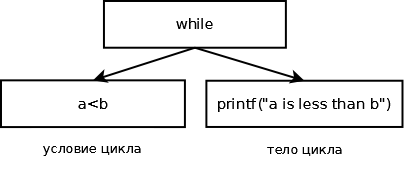
\includegraphics[width=\textwidth]{whileTree.png}
    \caption{Синтаксическое дерево.}
    \label{Дерево}
  \end{minipage}
\end{figure}

Помимо реализации синтаксического анализатора языка, часто реализуется так называемый pretty-printer, который в дальнейшем будет называть принтером, а сам процесс его работы -- печатью. Он позволяет получить текстовое представление программы на основе синтаксического дерева. Однако у программы может быть несколько представлений, и то, какой код получится, играет немаловажную роль. На рисунке 3 представлен код неотформатированной программы, на рисунке 4 тот же самый код, но уже с добавлением отступов, переносов строк, пробелов в 
определённых местах, что намного облегчает восприятие программы.

\begin{figure}[h]
\centering

\begin{verbatim}
    int foo(int a, int b){while(a<b)
    {printf("a is less than b")
    ;a=a+1;}return a;}
\end{verbatim}

\caption{Неотформатированная программа}
\label{Неотформат}
\end{figure}

\begin{figure}[h]
\centering

\begin{lstlisting}[language = C]
    int foo(int a, int b)
    {
        while(a<b)
        {
            printf("a is less than b");
            a = a+1;
        }
        return a;
    }
    
\end{lstlisting}

\caption{Форматированная программа}
\label{Отформат}
\end{figure}

%Таким образом, можно считать, что принтер и синтаксический анализатор выполняют обратные друг к другу функции.

%При разработке средств для языков программирования, помимо реализации синтаксического анализатора языка, часто реализуется так называемый pretty-printer, который в дальнейшем будет называть принтером. Принтер осуществляет обратное представление кода по синтаксическому дереву. Синтаксическое дерево строится синтаксическим анализатором на основе токенов, полученных лексическим анализатором, и представляет из себя древовидную структуру, в узлах которого находятся операторы, а в узлах-потомках -- аргументы оператора. Рассмотрим пример: на рисунке 1а представлен код программы, а на 1б -- синтаксическое дерево, соответствующее данному коду. 


%Принтер позволяет получить код программы по синтаксическому дереву, однако то, какой код получится, играет немаловажную роль. Рассмотрим очередной пример: на рисунке 2а представлен код неотформатированной программы, на рисунке 2б тот же самый код, но уже с добавлением отступов, переносов строк, пробелов в определённых местах, что намного облегчает восприятие программы. Принтер позволяет выводить хорошо форматированный код, и то, на сколько гибко можно варьировать количество отступов, пробелов, переносов строк, является одной из характеристик сравнения принтеров.

В большинстве случаев синтаксический анализатор и принтер никак не связаны между собой и являются двумя разными программами, хотя выполняют они функции, обратные друг к другу, то есть для них можно ввести следующий инвариант: пусть имеется синтаксический анализатор 
\lstinputlisting[language=Haskell, firstline=1, lastline=1]{printer.hs}
и принтер, 
\lstinputlisting[language=Haskell, firstline=2, lastline=2]{printer.hs}

Все строки, которые равны с точки зрения синтаксиса языка, будут давать одно и тоже синтаксическое дерево, однако по одному и тому же синтаксическому дереву принтер может получить разные строки, отличающиеся, например, количеством пробелов как на рисунках ~\ref{Неотформат}, ~\ref{Отформат}.
Из этого следует, что композиция синтаксического анализатора и принтера будет тождественной функцией, 
\lstinputlisting[language=Haskell, firstline=3, lastline=3]{printer.hs}
а обратная композиция не является тождетсвенной.
\lstinputlisting[language=Haskell, firstline=4, lastline=4]{printer.hs}

%Практика показывает, что синтаксический анализатор и принтер -- довольно сложные системы. Это связано с тем, что важным требованием является скорость их работы и корректность. Сложность реализации можно проследить на таких примерах, как принтер- и парсер-комбинаторы [ссылки]. Зачастую трудность реализации влечёт за собой не соблюдение инварианта принтера и синтаксического анализатора.

Для разработки синтаксических анализаторов и принтеров на языке Haskell довольно часто используются библиотеки и встраиваемые предметно-специфичные языки (embedded domain-specific languages, EDSLs). Например, стандартные библиотеки ghc включают в себя библиотеку Parsec, встроенный синтаксический анализатор DSL (Leijen и Meijer 2001) для синтаксического анализа, а также EDSL для реализации принтеров (Hughes 1995). Эти библиотеки независимы между собой и сложны в реализации, так как от них требуется высокая скорость работы и корректность. Все это влечёт за собой несоблюдение инварианта принтера и синтаксического анализатора.

Возникает вопрос о совместном задании принтера и синтаксического анализатора. У этого подхода есть ряд положительных качеств. Во-первых, это позволит не реализовывать две схожие программы отдельно. Как следствие, уменьшается вероятность появления ошибок, связанных с их инвариантом. Кроме того, такой подход позволит не переносить изменения, сделанные в одном из компоненте, на другой. Во-вторых, все строки, которые генерируются принтером, корректно воспринимаются синтаксическим анализатором. В-третьих, инвариантность принтера и синтаксического анализатора получается автоматически за счёт задания их как единой структуры.

В данной работе были рассмотрены три статьи, предоставляющие возможности совместного задания принтера и синтаксического анализатора для формальных языков ~\cite{Rendel}, ~\cite{Matsuda}, ~\cite{Boespflug}.

Целью данной работы является обзор существующих статей в данной предметной области, выявление их положительных и отрицательных сторон, а именно: как сильно можно варьировать вывод принтера, можно ли использовать параметры вывода, например, ширина. Для этих целей на основе каждой статьи реализуется синтаксический анализатор и принтер для учебного языка L. На рисунках~\ref{lol1},~\ref{lol2} показаны два различных представления кода в зависимости от того, какая ширина вывода.

\begin{figure}[h]
  \centering
  \begin{minipage}[h]{0.4\textwidth}
    \begin{lstlisting}[language = C]
printf("a is less than b"); a = b;
    \end{lstlisting}
    \caption{Представление программы при ширине вывода больше 34}
    \label{lol1}
  \end{minipage}
  \hfill
  \begin{minipage}[h]{0.4\textwidth}
    \begin{lstlisting}[language = C]
printf("a is less than b"); 
    a = b;
    \end{lstlisting}
    \caption{Представление программы при ширине вывода меньше 34}
    \label{lol2}
  \end{minipage}
\end{figure}



\section{Обзор статьи T. Rendel, K. Ostermann
}

Авторами данной статьи был разработан EDSL язык синтаксических дескрипторов (syntax descriptions) для объединения синтаксического анализа и печати, основанный на частичных изоморфизмах (partial isomorphisms), с помощью которых можно осуществлять обратимые вычисления. Авторы предоставляют интерфейс синтаксических дескрипторов как множество классов типов (type classes). Также они разработали единые комбинаторы для синтаксического анализа и печати.

Рассмотрим пример. На рисунке~\ref{AST} представлен результат обработки строки "((SK)K)" на языке \lstinline[language=haskell,mathescape]{data SK = S | K | App SK SK} синтаксическим анализатором.
\begin{figure}[h]
  \centering
    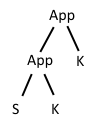
\includegraphics[scale = 0.9]{AST.png}
    \caption{Синтаксическое дерево.}
    \label{AST}
 \end{figure}

Программа, реализующий синтаксический анализатор и принтер выглядит следующим образом.

\begin{figure}[h]
\label{разрыв_функции}
\centering

\begin{lstlisting}[language = Haskell]
    parserSK = exp1 where
        exp0 = s <$ tok "S"
           <|> k <$ tok "K" 
           <|> tok "(" *> exp1 <* tok ")"
        exp1 = foldl app <$> exp0 <*> many exp0
        tok k = string k <* spaces
    
\end{lstlisting}

\caption{Синтаксический анализатор и принтер}
\end{figure}

%Для начала рассмотрим комбинаторы <\$>, <*>, <|>, как если бы они были реализованы в программе, которая осуществляет лишь синтаксический анализ.

Рассмотрим комбинатор (<\$>), как если бы он был реализован в библиотеке, которая осуществляет лишь синтаксический анализ. Этот комбинатор имел бы тип
\lstinline[language=haskell,mathescape]{$(\alpha \rightarrow \beta) \rightarrow (Parser $ $\alpha \rightarrow Parser$ $ \beta)$}
%\begin{lstlisting}[mathescape]
%$(<\$>) :: (\alpha \rightarrow \beta) \rightarrow (Parser $ $\alpha \rightarrow Parser$ $ \beta)$
%\end{lstlisting}
и позволял бы получить синтаксический анализатор некоторого типа $\beta$, имея синтаксический анализатор типа $\alpha$ и функцию из $\alpha$ в $\beta$. Теперь рассмотрим этот же комбинатор с точки зрения принтера. Он имел бы тип \lstinline[language=haskell,mathescape]{$(\beta \rightarrow \alpha) \rightarrow (Printer $ $\alpha \rightarrow Printer$ $ \beta)$}


%\begin{lstlisting}[mathescape]
%$(<\$>) :: (\beta \rightarrow \alpha) \rightarrow (Printer $ $\alpha \rightarrow Printer$ $ \beta)$
%\end{lstlisting}
Как видно, два типа очень похожи, за исключением того, что в одном случае первый аргумент имеет тип $\alpha \rightarrow \beta$, а во втором $\beta \rightarrow \alpha$.

%Комбинатор <*>, имеющий следующий тип
%\begin{lstlisting}[mathescape]
%$(<*>) :: Parser $ $(\alpha \rightarrow \beta) \rightarrow (Parser$ $\alpha %\rightarrow Parser $ $ \beta)$
%\end{lstlisting}
%позволял бы комбинировать несколько синтаксических анализаторов последовательно.

%Комбинатор <|>, имеющий следующий тип
%\begin{lstlisting}[mathescape]
%$(<|>) :: Parser $ $\alpha \rightarrow Parser$ $\alpha \rightarrow Parser $ $ \alpha$
%\end{lstlisting}
%позволял бы комбинировать несколько синтаксических анализаторов как альтернативные друг к другу.

%Теперь рассмотрим эти же комбинаторы с точки зрения печати. Они имели бы следующие типы.
%\begin{lstlisting}[mathescape]
%$(<\$>) :: (\beta \rightarrow \alpha) \rightarrow (Printer $ $\alpha \rightarrow Printer$ $ \beta)$
%\end{lstlisting}

%\begin{lstlisting}[mathescape]
%$(<*>) :: Printer $ $\alpha \rightarrow Printer$ $\beta \rightarrow Printer $ $ (\alpha,\beta)$
%\end{lstlisting}

%\begin{lstlisting}[mathescape]
%$(<|>) :: Parser $ $\alpha \rightarrow Parser$ $\alpha \rightarrow Parser $ $ \alpha$
%\end{lstlisting}

Для обобщения комбинаторов для синтаксического анализа и печати авторами вводится понятие частичного изоморфизма. Заводится конструктор типа данных Iso, такой, что Iso $\alpha$ $\beta$ это тип частичного изоморфизма между  $\alpha$ и $\beta$
\begin{lstlisting}[mathescape,language = haskell]
data Iso $\alpha$ $\beta$
    = Iso($\alpha$ $\rightarrow$ Maybe $\beta$) ($\beta$ $\rightarrow$ Maybe $\alpha$)
\end{lstlisting}
Слово частичный здесь не случайно, как видно из определения конструктора Iso \textit{f g}, функции \textit{f} и \textit{g} по входному параметру могут получить Nothing. 

Теперь функции могут быть использованы как вперед, так и в обратную сторону. Например, модифицированный комбинатор <\$>, выглядящий следующим образом:

\begin{lstlisting}[mathescape]
$(<\$>) :: Syntax $ $\delta \Longrightarrow Iso$ $\alpha $ $ \beta \rightarrow (\delta $ $ \alpha \rightarrow \delta $ $\beta)$
\end{lstlisting}
выполняющий следующие функции: $f$<\$>$p$ синтаксический анализатор будет использовать функцию $f$ вперед для того, чтобы конвертировать значения после синтаксического анализа, а $f$<\$>$p$ принтер будет использовать $f$ в обратную сторону перед печатью. Однако, не все функции могут быть использованы при частичном изоморфизме, а только те, которые могут быть обратимы. Например, авторы реализуют обратимую функцию свёртки

\begin{lstlisting}[mathescape,language = haskell]
foldl :: ($\alpha$ $\rightarrow$ $\beta$ $\rightarrow$ $\alpha$) $\rightarrow$ $\alpha$ $\rightarrow$ $[\beta]$ $\rightarrow$ $\alpha$
\end{lstlisting}

\begin{lstlisting}[mathescape,language = haskell]
foldl ::  Iso ($\alpha$, $\beta$) $\alpha$ $\rightarrow$  Iso($\alpha$, $[\beta]$) $\alpha$
\end{lstlisting}
При обращении функции \textbf{foldl} конструкторам типа Iso получится функция \textbf{unfoldl}

Таким образом, авторами был разработан интерфейс, который позволяет совместно задать синтаксический анализатор и принтер (см. рисунок~\ref{КлассСинтДеск}).
\begin{figure}[ht]
\centering
\begin{lstlisting}[mathescape,language = haskell]
class (IsoFunctor $\delta$, ProductFunctor $\delta$, Alternative $\delta$) 
    => Syntax $\delta$ where
   -- $(<\$>)$  ::  Iso $\alpha$ $\beta$ $\rightarrow$ $\delta$ $\alpha$ $\rightarrow$ $\delta$ $\beta$
   -- $(<*>)$   ::  $\delta$ $\alpha$ $\rightarrow$ $\delta$ $\beta$ $\rightarrow$ $\delta$ ($\alpha$, $\beta$)
   -- $(<|>)$   ::  $\delta$ $\alpha$ $\rightarrow$ $\delta$ $\alpha$ $\rightarrow$ $\delta$ $\alpha$
   -- empty   ::  $\delta$ $\alpha$
   pure   ::  Eq $\alpha$ => $\alpha$ $\rightarrow$ $\delta$ $\alpha$
   token  ::  $\delta$ Char
\end{lstlisting}
\caption{Класс синтаксических дескрипторов}
\label{КлассСинтДеск}
\end{figure}

Дескриптор token связывает символ с самим собой, pure x в случае синтаксического анализа возвращает x, не требуя какого-либо ввода, а, в случае принтера, отбрасывает значения, равные x. Используя этот интерфейс, можно реализовать функцию, которая является и синтаксическим анализатором, и принтером.

В данном подходе никоим образом не задается вариативность принтера в зависимости от ширины вывода. Однако при реализации данного подхода для учебного языка L было выяснено, что можно задать функцию от булевого флага, с помощью которой можно варьировать количество пробелов, переносов строк, отступов. Ниже представлена часть программы, реализующий флаг, и пример работы этого флага. 


\begin{figure}[ht]
\centering
\begin{verbatim}

optSpace' :: Syntax delta => Bool -> delta ()
optSpace' True  =  ignore [()]  <$>  (many (text "\n   ") <|> many (text " "))
optSpace' False =  ignore [()]  <$> (many (text " ") <|> many (text "\n"))

statement = stm 1 where
    stm 0 = readStm <$> readstm
        <|> write <$> write'
        <|> while <$> while'
        <|> ifExp <$> ifexp

    stm 1 = (seqStm <$> (stm 0 <*> text ";" *> stm 1))
	        <|> stm 0
    readstm = keyword "read"
            *> parens (identifier)
    write'  = keyword "write"		  
            *> parens (expression)
    while' = keyword "while"
            *> parens (expression) <*> optSpace' False *> (statement)
    ifexp  = keyword "if"
            *> optSpace  *> parens (expression)
                                    <*> optSpace  *> (statement) 
                                    <*> optSpace  *> keyword "else"  
                                     *> optSpace  *> (statement)	

\end{verbatim}
\caption{Реализация булевого флага}
\label{БулФлаг1}
\end{figure}

При выставлении у функции optSpace' параметра True, происходит форматирование, как на рисунке~\ref{True}, а при параметре False, как на рисунке~\ref{False}

\begin{figure}[h]
  \centering
  \begin{minipage}[h]{0.4\textwidth}
    \begin{lstlisting}[language = C]
    while(1)
       read(x)
    \end{lstlisting}
    \caption{Флаг равен True}
    \label{True}
  \end{minipage}
  \hfill
  \begin{minipage}[h]{0.4\textwidth}
    \begin{lstlisting}[language = C]
    while(1) read(x)
    \end{lstlisting}
    \caption{Флаг равен false}
    \label{False}
  \end{minipage}
\end{figure}


%Был разработан синтаксический анализатор и принтер для учебного языка L. Было выяснено, что количество пробелов, переносов строк, отступов можно варьировать, причём это можно реализовать с помощью булевого флага. Из этого можно сделать вывод, что при желании можно реализовать ввод параметров для количества отступов, пробелов, переносов. Ниже представлен пример работы этого флага.

Однако мы стремимся получить вариатиность не от булевого флага, а в зависимости от ширины вывода. Для того, чтобы появилась такая возможность, нужно либо придумывать более сложные структуры, нежели флаг, либо обернуть получение параметров вывода в монадные вычисления. Однако функции, осуществляющие данные вычисления, довольно трудоёмко реализовать обратимыми.

Одним из ограничений данного метода является использование расширений 
TemplateHaskell, NoMonomorphismRestriction, RelaxedPolyRec языка Haskell.
%В ходе работы был произведён замер производительности реализации синтаксического анализатора и принтера для учебного язык L. На входе из 512 операторов скорость работы варьировалась в границах 0.21 -- 0.27 секунд, в среднем 0.23 секунды.

%У подхода, предложенного в данной статье, есть ряд ограничений. Частичный изоморфизм может быть реализован только с обратимыми функциями. Это влечёт за собой более важную для нас проблему, а именно то, что принтер не может продуцировать представления, зависящие от раскладки, а именно от ширины вывода, так как функции Haskell, позволяющие получить эти данные, не являются обратимыми.



\section{Обзор статьи K. Matsuda M. Wang
}

В данной статье авторы разработали систему FliPpr для получения синтаксического анализатора из принтера. Одним из важных элементов системы FliPpr является язык Surface Language, оснащённый комбинаторами библиотеки Вадлера для печати~\cite{WadlerPrinter}, с помощью которого реализуется принтер. Далее программа на языке Surface Language преобразуется в язык Core Language с помощью системы FliPpr. Следующим этапом работы системы является генерация контексно-свободной грамматики по программе на Core Language. В итоге полученная грамматика передается парсер-генератору и получается синтаксический анализатор (рис.~\ref{схемаFliPpr})

\begin{figure}[h]
\centering
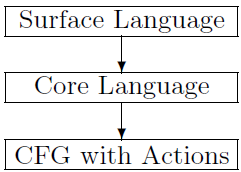
\includegraphics{FliPprScheme.png}
\caption{Схема работы FliPpr}
\label{схемаFliPpr}
\end{figure}



Рассмотрим работу систему FliPpr на примере. На рисунке ~\ref{Пример_принтера} представлен принтер для небольшого языка \lstinline[language=haskell,mathescape]{data E = Sub E E | One}.
\begin{figure}[h]
\centering
\begin{lstlisting}
ppr x = ppr x <+ text "(" <> nil <> ppr x <> nil <> text ")"
ppr One = text "1"
ppr (Sub e1 e2) = group (ppr e1 <> 
                  nest 2 (line' <> text "-" <> space' <> pprP e2))
pprP x = pprP x <+ text "(" <> nil <> pprP x <> nil <> text ")"
pprP One = text "1"
pprP (Sub e1 e2) = text "(" <> nil <> group (ppr e1 <> nest 2 (line'
                 <> text "-" <> space' <> pprP e2)) <> nil <> text ")"
space' = space <+ text ""
line' = line <+ text "" 
\end{lstlisting}
\caption{Пример принтера}
\label{Пример_принтера}
\end{figure}

Помимо вадлеровских комбинаторов для печати group, nest, авторами вводится комбинатор выбора (<+) (Biased Choice)
Он нужен для того, чтобы синтаксический анализатор мог воспринимать не только строчки, которые производит принтер. Принцип действия этого комбинатора следующий: когда программа воспринимается как принтер, то выполняется действие лишь левого операнда (<+). Однако с точки зрения синтаксического анализатора этот комбинатор интерпретируется как недетерменированный выбор, который принимает как левый, так и правый операнд. Например, можно определить количество пробелов и переносов строк следующим образом:
\begin{lstlisting}[mathescape]
$nil$ = $text$ "" <+ $space$
$space$ = ($text$ " " <+ $text$ "\n") <> $nil$
\end{lstlisting}
где $nil$ позволял бы воспринимать ноль или больше пробелов с переносом строки во время синтаксического анализа и получать ноль пробелов во время печати, а  $space$ позволял бы воспринимать один или больше пробелов с переносом строки во время синтаксического анализа и получать один пробел во время печати. Например, строки вида \lstinline{1    - 1, (1)-((1)), (1 - (1))} анализируются корректно.

Данный подход поулчения синтаксического анализатора из принтера основывается на предыдущей работе авторов об grammar-based inversion~\cite{MatsudaPrew}. Используя идеи из статьи~\cite{MatsudaPrew}, программа на языке Core Language может быть инвертирована для получения контекстно-свободной грамматики особого вида (CFG with actions)(см. рис.~\ref{Пример_CFGAct}) исходного языка. Далее в программе FliPpr авторами используется парсер-генератор, основанный на статье автора Frost и др.~\cite{Frost} для получения синтаксического анализатора. Однако для того, чтобы инверсия была возможна, на программу на языке Core Language накладываются ограничения, а именно программа должна быть linear и treeless~\cite{WadlerDeforest}. Вследствие этих ограничений, нельзя релизовать хороший принтер с гибкими настройками форматирования, поэтому был разработан Surface Language, но уже без выше указанных ограничений, дающий возможности хорошей печати, а далее с помощью техник програмной трансформации deforestation~\cite{WadlerDeforest} и др. программа на языке Surface Language переводится в программу на Core Language.


\begin{figure}[h]
\centering
\begin{lstlisting}[mathescape]
PPr $\rightarrow$ Ppr_                 {$\textdollar$ 1}
    | "(" Nil Ppr Nil ")" {$\textdollar$ 3} 
Ppr_$\rightarrow$ 1                          {$\textdollar$ One}
    | Ppr Line' "-" Space' PprP {Sub $\textdollar$1 $\textdollar$5 }
...    
\end{lstlisting}
\caption{Пример CFG with actions}
\label{Пример_CFGAct}
\end{figure}

На рисунке~\ref{ЯзыкLFliPpr} представлена часть реализации принтера на яыке Surface Language для учебного языка L, которая обрабатывает цикл while.
\begin{figure}[ht]
\centering
\begin{lstlisting}
ppr' i d (ExWhileZ _ x y ) = parensIf (d == L) $ group $ 
    text "while" <> nil <> space' <> ppr 0 R x <> line <> 
    text "do" <> space <> nest 3 (ppr 0 R y);
                                                
parensIf b d = if b then parens d else d ;
manyParens d = d <+ parens (manyParens d);
parens d = text "(" <> nest 1 (nil <> d <> nil) <> text ")";
space = (text " " <+ charOf (spaceChars `butnot` char ' ')) <> nil;
nil = text "" <+ (charOf spaceChars <> nil);
\end{lstlisting}
\caption{Обработка цикла while для языка L}
\label{ЯзыкLFliPpr}
\end{figure}

Достоинством данного метода является то, что для принтера используются комбинаторы из библиотеки Вадлера. Это предоставляет широкие возможности для форматирования, в том числе с использование ширины вывода. Также стоит отметить вариативность в плане выбора парсер-генератора. Однако ограничения, которые накладываются на Core Language, могут в перспективе вызвать ограничения при реализации синтаксических анализаторов и принтеров для сложных структур.


\section{Обзор статьи M. Boespflug
}

В данной статье авторы представляют EDSL c семейством обратимых комбинаторов для совместного задания синтаксического анализа и печати. 

Для реализации данного подохода авторы разработали тип под названием кассета (Cassette). Кассета состоит из двух треков, которые представлены функциями.
\begin{lstlisting}[mathescape,language = haskell]
data K7 a b c d = K7 { sideA :: a -> b, sideB :: d -> c }
\end{lstlisting}
Кассеты можно склеивать, для получения новых.
\begin{lstlisting}[mathescape,language = haskell]
(<>) :: K7 b c b' c' -> K7 a b a' b' -> K7 a c a' c'
$\sim$(K7 f f') <> $\sim$(K7 g g') = K7 (f . g) (g' . f')
\end{lstlisting}

Кассета, которая на стороне А содержит синтаксический анализатор, продуцирующий данные типа а, и котора на стороне B имеет принтер данных типа а, называется P/P парой:
\begin{lstlisting}[mathescape,language = haskell]
type PP a = forall r r'. K7 (C (a -> r)) (C r) (C (a -> r')) (C r')
\end{lstlisting}
где конструктор C имеет тип \lstinline[language=haskell]{type C r = (String -> r) -> String -> r}

С кассетами можно делать следующие действия. Их можно проиграть:
\begin{lstlisting}[mathescape,language = haskell]
play :: K7 a b c d -> a -> b
play csst = sideA csst
\end{lstlisting}
Можно поменять стороны A и B местами:
\begin{lstlisting}[mathescape,language = haskell]
flip :: K7 a b c d -> K7 d c b a
flip (K7 f g) = K7 g f
\end{lstlisting}

Простейший синтаксический анализатор из кассеты получается следующим образом:
\begin{lstlisting}[mathescape,language = haskell]
parse :: PP a -> String -> Maybe a
parse csst = play csst (\_ _ x -> Just x) (const Nothing)
\end{lstlisting}

Если перевернуть кассету, то получится принтер:
\begin{lstlisting}[mathescape,language = haskell]
pretty :: PP a -> a -> Maybe String
pretty csst = play (flip csst) (const Just) (\_ _ -> Nothing) ""
\end{lstlisting}

Комбинатор (<|>) позволяет выбирать последовательно между несколькими кассетами. Если одна из них, например, не может проанализировать входную строку, то выбирается следующая кассета.
\begin{lstlisting}[mathescape,language = haskell]
(<|>) :: PP a -> PP a -> PP a
K7 f f' <|> K7 g g' =
  K7 (\k k' s -> f k (\s' -> g k k' s) s)
     (\k k' s x -> f' k (\s' -> g' k k' s) s x)
\end{lstlisting}

Основной особенностью данного подхода является то, что симметричность синтаксического анализатора и принтера реализуется с помощью задания их индуктивно (Continuation-passing style, CPS). По мнению авторов, такой способ задания комбинатора выбора (<|>) показывают более лучшие результаты в плане производительности, нежели c помощью методов, описанных в первой статье~\cite{Rendel}, где были использованный вложенные кортежи. 

Данный метод никак не позволят варьировать работу принтера в зависимости от ширины вывода. Как и в случае с первой статьей, был реализован синтаксический анализатор и принтер с булевым флагом, в зависимости от которого продуцировался разный вывод. Ниже представлена часть программы, реализующая флаг и результаты работы программы в зависимости от параметра.

\begin{figure}[ht]
\centering
\begin{verbatim}

optSpace' ::  Bool -> PP0
optSpace' True = unshift "\n   " $ many (satisfy isSpace)
optSpace' False = unshift " " $ many (satisfy isSpace)

stmnt :: PP Stmt
stmnt =   seqL    -->
          parens(stmnt<> optSpace <> string ";" <> optSpace <> stmnt)
      <|> readL   -->
          string "read" <> parens(ident)
      <|> writeL  -->
          string "write" <> parens(optSpace <> mainExpr <> optSpace)
      <|> whileL  -->
       string "while" <> parens(optSpace <> mainExpr <> optSpace) <> optSpace' True <> 
       optSpace <> stmnt <> optSpace 
      <|> assignL --> 
          ident <> optSpace <> string "=" <> optSpace <> mainExpr  
          

\end{verbatim}
\caption{Реализация булевого флага}
\label{БулФлаг2}
\end{figure}

При выставлении у функции optSpace' параметра True, происходит форматирование, как на рисунке~\ref{True}, а при параметре False, как на рисунке~\ref{False}.

\begin{figure}[h]
  \centering
  \begin{minipage}[h]{0.4\textwidth}
    \begin{lstlisting}[language = C]
    while( 1 )
       read(x)
    \end{lstlisting}
    \caption{Флаг равен True}
    \label{True}
  \end{minipage}
  \hfill
  \begin{minipage}[h]{0.4\textwidth}
    \begin{lstlisting}[language = C]
    while( 1 ) read(x)
    \end{lstlisting}
    \caption{Флаг равен false}
    \label{False}
  \end{minipage}
\end{figure}

Ограничением данного подхода является то, что он использует расширение RankNTypes языка Haskell.

\section{Сравнение предложенных подходов}
Методы, предложенные в первой и третьей статье, являются похожими друг на друга, у обоих методов совпадают некоторые комбинаторы, в обоих случаях никак не используются параметры вывода. Проблема обратимости функций, описанная в первой статье, была решена в третьей за счёт задания синтаксического анализатора и принтера в CPS. Однако оба этих метода используют некоторые расширения языка Haskell. Во второй статье используется другая концепция с использованием вадлеровских комбинаторов для печати, которая предоставляет большие возможности для вариативности принтера, в том числе и параметры ввода и вывода.
\begin{center}
    \begin{tabular}{ | p{4cm} | p{4cm} | p{3cm} | p{4cm} |}
    \hline
      & Syntax Descriptions & FliPpr & Cassette \\ \hline
    Использование ширины вывода & Нет & Да & Нет \\ \hline
    Что нужно реализовать & Cинтаксический анализатор  & Принтер & Cинтаксический анализатор \\ \hline
    Язык L (строк кода) & Около 250 & Около 60 & Около 230 \\ \hline
    Ограничения & Использование расширений языка Haskell, обратимость функций & Ограничения на Core Language & Использование расширений языка Haskell\\
    \hline
    \end{tabular}
\end{center}

Также авторами третьей статьи утверждалось, что их подход лучше подхода, описанного в первой статье, в плане производительности. Для проверки данного предположения был произведён замер скорости работы реализаций для языка L.
Для каждой программы генерировалось одинаковое синтаксическое дерево с разным количеством элементов. Замер производился отдельно для синтаксического анализа и печати. Результаты представлены в таблице ниже.


\begin{figure}[ht]
\centering
\begin{center}
    \begin{tabular}{ | p{4cm} | p{4cm} | p{3cm} | p{4cm} |}
    \hline
      & Syntax Descriptions &  Cassette \\ \hline
    100 элементов  & 3.1127e-2 & 1.092e-3 \\ \hline
    1000 элементов & 1.228305 & 7.031e-3    \\ \hline
    2000 элементов & 5.772979 & 1.3437e-2 \\
    \hline
    \end{tabular}
\end{center}
\caption{Производительность для синтаксического анализа}
\end{figure}



\begin{figure}[ht]
\centering
\begin{center}
    \begin{tabular}{ | p{4cm} | p{4cm} | p{3cm} | p{4cm} |}
    \hline
      & Syntax Descriptions &  Cassette \\ \hline
    100 элементов  & 5.282e-3 & 9.91e-4 \\ \hline
    1000 элементов & 3.2422e-2 & 1.0082e-2 \\ \hline
    10000 элементов & 0.452966 & 8.1065e-2 \\
    \hline
    \end{tabular}
\end{center}
\caption{Производительность для печати}
\end{figure}

Как видно из таблиц, предположения авторов третьей статьи об улучшении производительности подтвердились.

% У заключения нет номера главы
\section*{Заключение}
В данной работе представлен обзор статей на тему совместного задания синтаксического анализатора и принтера.
Было выяснено, что только один из подходов использует параметры вывода, например ширину. Для каждой из статей был реализован синтаксический анализатор и принтер для учебного языка L и было выяснено, что некоторая вариативность для двух других методов может быть задана, однако она никак не использует параметры вывода. Также был произведён замер производительности двух подходов для подтверждения улучшения производительности.


\bibliographystyle{ugost2008ls}
\bibliography{diploma.bib}
\end{document}
